% Chapter 3

\chapter{技术路线及预测结果} 
\label{Chapter3}  
\section{技术方案选择}
\subsection{理论基础}
对于信令数据可以采取一下两种向量化方法:
\begin{equation}
\begin{split}
p = & f(id,time,week[weather,air condition,...])\\
p = & f(id,time,week,p(last hour),p(yesterday),p(last week),p(last month))
\end{split}
\end{equation}
其中,p 代表人口数据,可以通过维度的不同进行不同的表达(一维表示驻留人数,三维表示驻留人数,出发人数和到达人数),特别的,id 中隐含了地域的信息。
\subsection{分析手段}
采用有监督人工神经网络,期望输出为驻留人数、出发人数、到达人数,其基本架构如图(\ref{fig:3.1})所示。
\begin{figure}[ht]
\centering
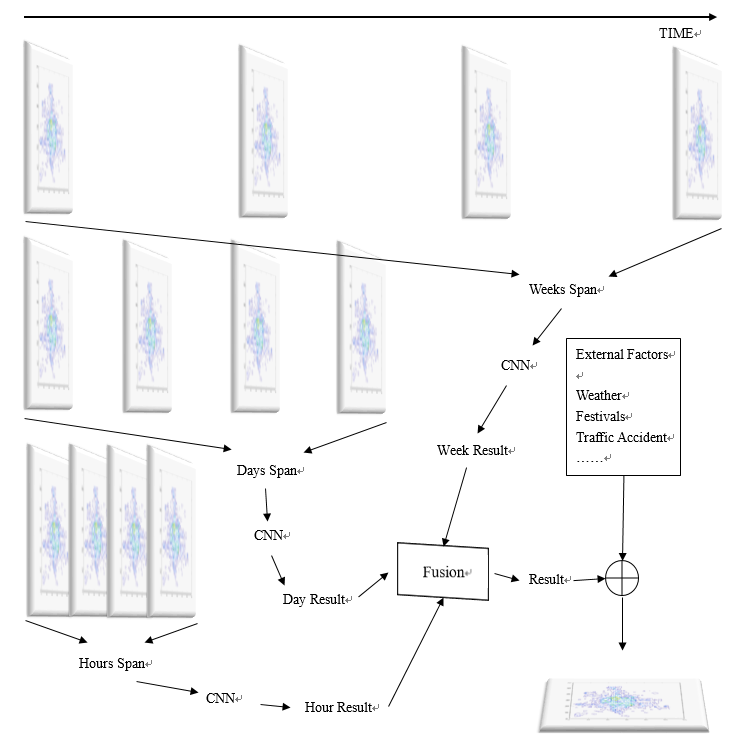
\includegraphics[width=0.8\textwidth]{ournet.png}
\caption{网络搭建基本构型}
\label{fig:3.1}
\end{figure}
输入为数据的特征,人工选取:我们认为主要以人数与 星期几(已有)、具体小时(已有)、位置(已有)、天气(可以爬取)、前一小时的人数(对已有数据处理)等主要因素有关。
同时我们以获得数据中的驻留人数、出发人数、到达人数作为标签,期望输出。
利用期望输出与网络输出之间的误差建立学习信号反向传播,修正网络权重。
\subsubsection*{初步网络搭建}
中间两个隐层,每个隐层20个神经元,采取全连接。
虽然说基站数量为2265个,我们的网络权重大约是600个待定参数好像不太够保存所有基站的信息。但是,注意到我们关注的是一片区域的总人口数据,而不是特指
某个基站的总人口个数,所以我们的网络只要区分出这种大概有同一人口特性的区域即可,最终对人口驻留,流动的分析也是基于区域进行分析的,所以600个左右的待定参数是够用的。
\subsubsection*{两种可能方案}
\begin{itemize}
	\item 方案A:多输入多输出(针对所有点的神经网络模型)\\
	类似于图片处理,2265个基站,输入即为2265*n,其中n为输入特征(星期,小时,ID(位置特征)等),输出为2265*3,3为标签个数(驻留人数、出发人数、到达人数)
	\item 方案B:少输入少输出(针对某一点的神经网络模型)\\
	针对某一个基站或者某一块区域进行训练。输入为特征个数(星期,小时,ID等),输出为3,即驻留人数、出发人数、到达人数。\\
	训练出来的模型是针对某一个基站或者某一块区域(9个基站左右,表示$9km^2$的一个区域)的人口情况。做分析时候要训练多点得到一个区域的数据进行分析。\\
	统计关心区域的总人口驻留,总人口流出,总人口流入来表示这个区域的人口数据。因为守恒关系,一个区域内所有点的人口驻留人数代数和即为该区域的总人口驻留人数,总人口流入与总人口流之差,即为该区域的总人口流入或总人口流出。
\end{itemize}
\subsubsection*{目前进度}
现已完成少输入少输出神经网络模型的搭建
\begin{itemize}
  \item 输入层:3个神经元输入
  \item 中间1层:20个神经元,激活函数ReLu
  \item 中间2层:20个神经元,激活函数ReLu
  \item 输出层:3个神经元输出(驻留人数,出发人数,到达人数)
\end{itemize}
用梯度下降方法、以及滑动平均,对训练进行优化。目前采用固定学习率训练,看效果之后可以采用指数下降学习率方法。
